%\documentclass[wcp,gray]{jmlr} % test grayscale version
%\documentclass[wcp]{jmlr}% former name JMLR W\&CP
\documentclass[pmlr]{jmlr}% new name PMLR (Proceedings of Machine Learning)

% The following packages will be automatically loaded:
% amsmath, amssymb, natbib, graphicx, url, algorithm2e

%\usepackage{rotating}% for sideways figures and tables
\usepackage{longtable}% for long tables

% The booktabs package is used by this sample document
% (it provides \toprule, \midrule and \bottomrule).
% Remove the next line if you don't require it.
\usepackage{booktabs}
% The siunitx package is used by this sample document
% to align numbers in a column by their decimal point.
% Remove the next line if you don't require it.
\usepackage[load-configurations=version-1]{siunitx} % newer version
%\usepackage{siunitx}

\makeatletter
\def\set@curr@file#1{\def\@curr@file{#1}} %temp workaround for 2019 latex release
\makeatother

% The following command is just for this sample document:
\newcommand{\cs}[1]{\texttt{\char`\\#1}}

% Define an unnumbered theorem just for this sample document:
\theorembodyfont{\upshape}
\theoremheaderfont{\scshape}
\theorempostheader{:}
\theoremsep{\newline}
\newtheorem*{note}{Note}

% change the arguments, as appropriate, in the following:
\jmlrvolume{126}
\jmlryear{2021}
\jmlrworkshop{Machine Learning for Healthcare}

% Short headings should be running head and authors last names
% \ShortHeadings{A Really Awesome MLHC Article}{Lastname, PhD and Lastname, MD}
% \firstpageno{1}

\title[Diagnosing Brain Disorders with Deep Anomaly Detection]{Diagnosing Brain Disorders with Deep Anomaly Detection}


\author{Amr Farahat$^{1 \star}$, Diyuan Lu$^{1 \star}r$, Sebastian Bauer$^{2}$, Valentin Neubert$^{3}$, Lara Costard$^{4}$, Felix Rosenow$^{2}$, Jochen Triesch$^{1, 2}$ \\
\small $^{1}$Frankfurt Institute for Advanced Studies (FIAS), Frankfurt am Main, 60438, Germany \\
\small $^{3}$Center for Personalized Translational Epilepsy Research (CePTER), Frankfurt am Main, Germany \\
\small $^{4}$Universitätsmedizin Rostock , Oscar-Langendorff-Institut für
Physiologie, Gertrudenstraße 9, Germany, Rostock, Germany\\
\small $^{5}$Tissue Engineering Research Group, Royal College of Surgeons Ireland, St Stephans Green 123, Dublin, D02, Ireland \\
}
\author{\Name{Amr Farahat$^{1}$}
\Email{farahat@fias.uni-frankfurt.de}\\ 
\AND
\Name{Diyuan Lu$^{1}$}
\Email{elu@fias.uni-frankfurt.de}\\ 
\AND
\Name{Sebastian Bauer$^{2}$}
\Email{Sebastian.Bauer@kgu.de}\\ 
\AND
\Name{Valentin Neubert$^{3}$}
\Email{valentin.neubert@uni-rostock.de}\\ 
\AND
\Name{Lara Sophie Costard$^{4}$}
\Email{laracostard@rcsi.com}\\ 
\AND
\Name{Felix Rosenow$^{2}$}
\Email{rosenow@med.uni-frankfurt.de}\\ 
\AND
\Name{Jochen Triesch$^{1, 2}$}
\Email{triesch@fias.uni-frankfurt.de}
\AND 
\small $^{1}$Frankfurt Institute for Advanced Studies (FIAS), Frankfurt am Main, 60438, Germany \\
\small $^{2}$Center for Personalized Translational Epilepsy Research (CePTER), Frankfurt am Main, Germany \\
\small $^{3}$Oscar Langendorff Institute of Physiology, Rostock University Medical Center, Rostock, Germany\\
\small $^{4}$Tissue Engineering Research Group, Royal College of Surgeons Ireland, St Stephans Green 123, Dublin, D02, Ireland \\
} 


%\editor{Editor's name}

\begin{document}

\maketitle

\begin{abstract}
	We consider a generalizable framework for diagnosing brain disorders from EEG recordings, in which a generative model is trained with EEG data from normal states to detect any systematic deviations from the normal signals. Early diagnosis of latent epileptogenesis (EPG) in epilepsy development prior to the first spontaneous seizure (FSS) is crucial for the prognosis, however challenging, due to lack of reliable bio-markers and hard-to-obtain data annotations. In this work, we propose to reformulate the early diagnosis problem as an unsupervised anomaly detection task, in which we train an adversarial autoencoder (AAE) to learn to encode normal EEG data into a low-dimensional latent space with an imposed prior distribution. We define the anomaly score as a combination of the reconstruction error and the distance of latent representation to the prior. Our results show that, in a rodent epilepsy model, the anomaly score increases as a function of time after the induced brain injury until the occurrence of the first seizure which hints at a gradual epileptogenic process that changes the features of the EEG signals. We also analyze the effect of different losses to the EPG detection performance. In conclusion, we demonstrate that unsupervised learning methods can be used to automatically detect systematic drifts in brain activity patterns occurring over long time periods. This could facilitate rapid diagnosis of brain diseases and open the door for early interventions.
\end{abstract}

% TODO: what are the anomaly waveforms? Are they indicative?
\section{Introduction}
%XX is an important problem in ML and healthcare.  (Make
%sure that the clinicians can see the relevance! \emph{Unclear clinical
%	relevance is a major reason that otherwise strong-looking papers are
%	scored low/rejected.})
%
%Addressing this problem is challenging because XX.  (Make sure that
%you connect to the ML here.)  
%
%Others have tried, but XX remains tough.  (Acknowledge related work.)
%
%In this work, we...

% current situation, significance of early diagnosis of epilepsy
There is nearly 1\% of the world's population suffer from epilepsy and there is no pharmacological treatments that could prevent epilepsy. Roughly 30\% of these patients will become pharmaco-resistant \citep{kwan2000early}. To issue early medical interventions and treatments and provide the potential epilepsy patients a better chance of living seizure-free lives, it is critical to identify them before the first spontaneous seizure (FSS), which is the beginning of established epilepsy \cite{moshe2015epilepsy}. 
Usually, there is a clinically-silent phase after the initial brain injury, during which the brain is undergoing a cascade of changes both functionally and structurally. That is when epileptogenesis (EPG) occurs. The term epileptogenesis (EPG) is the process where the healthy brain transformed to epileptic brain, capable of generating spontaneous recurring seizures \cite{loscher2019holy, pitkanen2014past}. 
The task of detecting the presence of epileptogenesis (EPG) in the latent period is very challenging since the process of EPG is still not fully understood \cite{pitkanen2016advances}. The challenges are (1) it is extremely difficult to collect data specifically during the latent period. (2) individual responses to different brain injuries. (3) significantly individual representative features introduce huge variability. (4) there is no well-established EEG biomarker for epileptogenesis.

% machine learning and anomaly detection in general
Recently advances in machine learning (ML) and deep learning (DL) offer promising directions. Applying DL-based method to epilepsy research have delivered encouraging results. \cite{lu2020towards, lu2020staging, rizzi2019changes, MORE}. These studies were conducted in supervised learning fashion, where labels of data are required. However, in the case of detecting EPG, the well-annotated labels are hard to obtain, or not possible at all. How can we detect the presence of EPG without large annotated epileptogenic data?
Here, we proposed a more general framework for detecting brain disorders in a complete unsupervised fashion based on the idea of anomaly detection (AD), and we conducted experiment on a rodent mesial temporal lobe epilepsy model (m-TLE) \cite{costard2019electrical}. Specifically, we do anomaly detection with time series data, i.e., EEG recordings. 



%  Need more AD application cases
Anomaly detection with time series learns features of nominal data from time sequence data, such as in medical applications \cite{zhou2019beatgan}, industrial equipment malfunction detection \cite{su2019robust}, traffic monitoring \cite{shipmon2017time}. 


% AD models
Specially, encoder-decoder-based AD models have shown impressive performances in learning a compact latent representation of the input data, and the reconstruction error has been a common metric for anomaly detection \cite{zhou2019beatgan, kumagai2019transfer, malhotra2016lstm, abati2019latent, schlegl2017unsupervised, su2019robust, kim2019rap}. In various of cases, the reconstruction error is in conjunction with other metrics such as distances of the hidden representations along the pathway \cite{kim2019rapp}, discriminative loss of generated features \cite{schlegl2017unsupervised}, and log-likelihood term \cite{abati2019latent}. 

However, ?????
% why use adversarial autoencoder?

% anomlay detection with time series, especially evolving data
It is especially challenging because the EEG data is highly non-stationary, evolving through time, share large part of features with that from healthy brain. 


% anomlay detection with time series, especially evolving data


% the difference in medical anomaly detection with EEG

Specifically, our contributions can be summarized as follows:
\begin{itemize}
	\item We present a general framework for detecting brain disorders based on EEG data
	\item We test our approach with data from a mTLE rodent model and demonstrate ... 
	\item latent vector analysis 
	\item reconstruction error and distance to the learned BL distribution could be a good indicator for detection EPG
\end{itemize}


\subsection*{Generalizable Insights about Machine Learning in the Context of Healthcare}
This section is \emph{required}, must keep the above title, and should
be the final part of your introduction.  In about one paragraph, or
2-4 bullet points, explain what we should \emph{learn} from reading
this paper that might be relevant to other machine learning in health
endeavors.

For example, a work that simply applies a bunch of existing algorithms
to a new domain may be useful clinically but doesn't increase our
understanding of the machine learning and healthcare; if that study
also investigates \emph{why} different approaches have different
performance, that might get us excited!  A more theoretical machine
learning work may be in how it enables a new kind of clinical study.
\emph{Reviewers and readers will look to evaluate (a) the significance
	of your claimed insights and (b) evidence you provide later in the
	work of you achieving that contribution}




\section{Related work}
% good \cite{serra2019input} \cite{kim2019rapp}
\subsection{Early Diagnosis of Epilepsy with EEG}
Early diagnosis of epilepsy holds great potential to address early treatment that could alter the disease progression, ultimately, saving lives, improving life quality of patients, alleviating huge social and financial burdens. However, obtaining models that could capture EEG bio-markers relevant for epilepsy progression is challenging due to the lack of well-defined bio-markers and not well-known process. 

\cite{ELGER2018279} Diagnostic challenges in epilepsy: seizure under-reporting and seizure: 


There have been an increasing research interest in this area \cite{lu2020towards, lu2020staging, rizzi2019changes}. Rizzi \textit{et al.} investigated the nonlinear dynamics of EEG signals and found a significant decrease of the so-called embedding dimension in early EPG that correlates with the severity of the ongoing EPG \cite{rizzi2019changes}.
\cite{lu2020towards} approaches the early diagnosis of epilepsy by designing a supervised two-class classification problem where a deep residual network is trained to distinguish data take from different phases during EPG. The model is 
\cite{lu2020staging} further extended the problem of distinguishing EEG data from healthy phase and EPG phase to staging the progress of EPG during the latent period.

We propose a deep encoder-decoder-based model that aims to learn a manifold of nominal data before the disease-inducing brain injury.


\subsection{Anomaly Detection}
% General research on AD --> time series AD --> autoencoder-based (reconstruction-based) AD 
% anomaly score
% conventional anomaly detection
Anomaly detection (AD) is a class of problems of detecting unusual instances, which differ from the expected normal pattern. Many AD methods have been proposed such as one-class support vector machines (OSVMs) \cite{scholkopf2001estimating, tax2004suppor}, semi-supervised learning AD models \cite{ruff2019deep}, unsupervised learning AD models \cite{bibid}. Anomaly detection has been used in various application areas such as industrial \cite{bibid}, healthcare \cite{bibid}. Due to the difficulty to obtain labeled anomalous samples, AD is often done in unsupervised fashion. 
In the case of detecting early signs of ongoing epileptogenesis, it is hard to acquire the data in this specific time window. In comparison, the relative healthy brain EEG recordings could be obtained more easily.


Anomaly detection (AD) is one class of problems to detect samples that do not conform the regularity of the training data. It could be implemented in supervised learning, semi-supervised learing \cite{ruff2019deep}, or unsupervised learning fashion \cite{} given the availability of sample labels \cite{NEURIPS2019_805163a0}. It can be also viewed as one-class learning problem, where the training data are deemed to be the one class of interest. The models are trained on this class of data and used for detecting anomalies \cite{shen2020timeseries,ruff2019self,ruff2018deep, scholkopf2001estimating, tax2004support}. Two classic one-class classification models are the support vector data description (SVDD) \cite{tax2004support}, where the model tries to build a spherical boundary to describe the training data and was trained to minimize the volume of the sphere to detect outliers and the one-class support vector (OC-SVM) \cite{scholkopf2001estimating}, where they used a hyperplane to separate the normal data and the outliers. An improved version of the SVDD model is proposed in

very often the access to the normal data is easier and that of anomalous data is difficult . 



\cite{ruff2019deep} DEEP SEMI-SUPERVISED ANOMALY DETECTION: deepSAD, an end-to-end deep learning framework for semi-supervised anomaly detection, where the model is trained to maximize the mutual information between the input data and the latent representation and a discounted label representation that is based on entropy. 
More commonly, AD is done in an unsupervised fashion \cite{references}.

% classic anomaly detection OC-SVD, SSVD
% volume of sphere
\cite{tax2004support} Support vector data description (SVDD): proposed to build a spherical boundary to describe the training data and by minimizing the volume of the sphere to detect outliers.
\cite{ruff2018deep}%https://github.com/nuclearboy95/Anomaly-Detection-Deep-SVDD-Tensorflow
Deep one-class classification: consider a neural network trained to minimize the volume of the hypersphere where the data representation vector resides. (in our work, we try to map the latent representation of the healthy data points to a prior distribution through the GAN graining)
\cite{shen2020timeseries} Time series anomaly detection using temporal hierarchical one-class network: proposed a temporal hierarchical one-class network for time series anomaly detection, where a dilated recurrent neural network with skip connections is trained to capture temporal features in multiple scales. Then, multiple hypershperes are obtained through hierarchical clustering. The model is trained to minimize the distance of the encoded representation to be closer to the centroids of multi-scale-hyperspheres
\cite{gopalan2019pidforest} PIDForest: anomaly detection via partial identification: random-forest-based AD method, which partition the space into subcubes and the anomalous samples will lie in subcubes with high sparsity.

% Deep learning-based AD methods. reconstruction-error-based, latent-vector-added, adversarial network-based
Reconstruction-error-based AD models are very popular. These models are often trained with only nominal data and samples that can not be well reconstructed, i.e., with high reconstruction error, deemed to be anomalous \cite{kumagai2019transfer}.
\cite{kumagai2019transfer} Transfer anomaly detection by inferring latent domain representations: proposed a method that could transfer the knowledge learned with data from related domains to the target domain to infer anomaly through the latent domain vectors. The anomaly score is based on the reconstruction of the autoencoder.

% loglikelihood-based method
\cite{malhotra2016lstm} LSTM-based encoder-decoder for multi-sensor anomaly detection (): proposed a reconstruction-error-based AD detection method where a LSTM encoder-decoder network is trained to reconstruct nominal time series data. The reconstruction error is used to estimate parameters of a Normal distribution $\mathcal{N}(\mu, \Sigma)$ through maximum likelihood estimation.
\cite{hendrycks2016baseline} A baseline for detecting misclassified and out-of-distribution examples in neural networks: combining out-of-distribution detection with misclassification. The intuition is that the predicted probability of incorrect and out-of-distribution examples is often lower than that for correct examples.
\cite{abati2019latent}--latent space auto-regression for novelty detection: proposed a framework where a deep autoencoder equipped with a parametric density estimator, which could learn the probability distribution of the learned latent representations through an autoregressive procedure. In all experiments the novelty assessment on the i-th example is carried out by summing the reconstruction term (RECi) and the log-likelihood term (LLKi). 
\cite{schirrmeister2020understanding} Understanding anomaly detection with deep invertible networks through hierarchies of distributions and features-failure explanation: when the discriminative features between inliers and outliers are on a high-level problem. It is based on log-likelihood-ratio-based anomaly detection method.
\cite{serra2019input} Input complexity an out-of-distribution detection with likelihood-based generative models-failure explanation: proposed an efficient and parameter-free anomaly score based on the estimation of the input complexity since likelihood-based generative models sometimes fail to detect certain forms of anomalous inputs that significantly differ from the training data. The anomaly score is based on the negative log-likelihood and the complexity estimate of the input, expressed in bits per dimension.
\cite{ren2019likelihood} % show failure cases where model assign higher confidence to OOD than in-distribution
Likelihood ratios for out-of-distribution detection: proposed a likelihood ratio method, which trains a model to capture background statistics of known bacteria genome sequences in order to detect unseen bacteria. 

% latent-code-based
\cite{abati2019latent} general framework where we equip a deep autoencoder with a parametric density estimator that learns the probability distribution underlying its latent representations through an autoregressive procedure.
\cite{ruff2019self} self attentive, multi-context one-class classification for unsupervised anomaly detection on text: proposed context vector data description method which leverages the learned word embedding from the pretrained model to perform AD on text data. The anomaly score is defined as the cosine distance of the contextual embedding to the respective context vector.


% sparsity, covariance, volumn
\cite{shipmon2017time} Time series anomaly detection (noisy highly periodic data)-google: regression task to compare the predicted values and the ground truth. Use two sliding window to compute the mean and variance of the series of the difference between prediction and ground truth and the two sliding means and variance are used to compute the final anomaly score. 

% adversarial autoencoder based models
\cite{pidhorskyi2018generative} generative probabilistic novelty detection with adversarial autoencoders: encoder-decoder-based model, which is based on adversarial autoecoders. They leverage two discriminators to ensure the latent distribution and sample generation quality. 
\cite{schlegl2017unsupervised} Unsupervised anomaly detection with generative adversarial networks ot guide marker discovery: a deep convolutional generative adversarial network is trained to capture a manifold of normal anatomical variability in optical coherence tomography images of the retina. The anomaly score is defined as the weighted sum of residual loss, a measure of reconstruction error, and discrimination loss, a measure of how well the generated features match that of the training data. Different from \cite{schlegl2017unsupervised}.
Similar to our approach. Additionally, we have a more flexible framework to aggregate different losses and to ensure robust generation, we add noise in the latent vector such that noisy latent code could also produce reasonably good generation.


% time series anomaly detection
industrial application \cite{su2019robust}

\cite{su2019robust} Robust anomaly detection for multivariate time series through stochastic recurrent neural network: prediction reconstruction probability.


% reconstruction with feature matching in all layers
\cite{kim2019rapp} RaPP: Novelty detection with reconstruction along projection pathway: proposed a autoencoder-based AD method by comparing data not only in the input space but also in the embedding spaces. The anomaly score is defined as Euclidean distances between the query and the reconstruction as well as all pairs of hidden representation of those two along the pathway.
\cite{zhang2019deep},-A Deep Neural Network for Unsupervised Anomaly Detection and Diagnosis in Multivariate Time Series Data: the model characterizes system status with signature matrices, which represents the correlations between different pairs of time series at multi-scale resolution. Then spatial information is encoded through a conv-encoder and the temporal information is encoded by a attention-based convLSTM. The a conv-Decoder is implemented to reconstruct the signature matrices.






% survey of anomaly detection



However, in our case, the signal is gradually evolving, which reflects the underlying changes taking place in the brain turning a healthy brain into an epileptic one. 











% AD for medical applications
\cite{zhou2019beatgan} BeatGAN: anomalous rhythm detection using adversarially generated time series: a GAN-based model trained on normal ECG traces is used for ECG anomaly detection. The anomaly score is defined as reconstruction error between the generator's output of a given input sample.
\cite{kalinichenko2014methods} methods for anomaly detection-- a survey CURE workshop:	
\cite{hendrycks2018deep} Deep anomaly detection with outlier exposure: proposed a method called outlier exposure, which leverages an auxiliary dataset of outliers while training the main AD model to classify whether a query is from in-distribution set or out-distribution set.
\cite{2020Deep} Deep Learning for Medical Anomaly Detection -- A Survey: , 
\cite{Salem2013SensorFA} anomaly detection for medical data 


Inspired by \cite{makhzani2015adversarial}, our work is in the same line of research.



% special about the EEG data. TODO: semi-supervised anomaly detection, incorporating EEG expert knowledge in AD. Train a VAE with TUH The TUH EEG Events Corpus (TUEV) https://www.isip.piconepress.com/projects/tuh_eeg/html/downloads.shtml --> scan EEG into latent representation --> LSTM to take sequence of representation --> anomaly detection
In EPG EEG recordings, there are various waveforms that are present both in EPG and BL phases.


% Our work: its novelty: 
We not only measure the reconstruction error in the input space, we also impose a prior distribution for the encoded latent space. To ensure robust encoding of the input data given noisy settings, we also add noise to the latent vector and enforce the reconstruction of the noisy latent vector still close to the original clean data. We have multiple loss metrics and could potentially be extendable to various learning paradigms given different weights for different losses.



Novelties of our proposed method:
\begin{itemize}
	\item Anomaly detection in gradually evolving time series data
	\item network structure is based on adversarial autoencoder
	\item robust encoding by impose noise in adversarial generating latent code
	\item multiple loss metrics are weighted-aggregated together. Flexibility of been extended to different paradigms. 
\end{itemize}
Our model falls back to common-version of reconstruction-error based AD method when AE-loss-weight is 1 and others 0. \textbf{Other cases...}



\subsection{Adversarial Autoencoder - Amr}
Autoencoders are neural networks that aim at learning lower-dimensional representations of the data by being trained to reconstruct its input \cite{Hinton2006}. The network is formed of two parts: an encoder and a decoder. The encoder maps the input into lower-dimensional bottleneck, which the decoder uses to output a reconstructed version of the input. These networks can be turned into generative models by being trained to learn the parameters of a prior distribution to the latent space instead of the precise representations e.g. variational autoencoders (VAEs) which impose the prior distribution through Kullback–Leibler divergence loss \cite{Kingma2013}. Adverserial autoencoders (AAEs) extend this notion by imposing this prior through adversarial training, which allows for more flexibility in choosing the prior \cite{makhzani2015adversarial}. A discriminator network is trained simultaneously to differentiate between real samples drawn from the prior distribution and the output of the encoder, which is additionally trained to fool the discriminator.  



% It would be great to get a trajectory in the latent space 
\section{Data}
\subsection{Dataset - Diyuan}\label{dataset}
% \begin{figure}[tb]
% 	\centering
% 	\includegraphics[width=0.9\linewidth]{figures/time-span.pdf}
% 	\caption{Schematic of the timeline of the experiment. A. time line for PPS-stimulated rats. B: time line for control rats.
% 		PPS: perforant pathway stimulation. FSS: first spontaneous seizure. The mean and standard deviation of the duration of EPG in the PPS group is $23.7 \pm 15.5$ days (min.\ 10 days, max.\ 56 days).}
% 	\label{timespan}
% \end{figure}
% \label{dataset}

We used continuous intracranial EEG data recorded by a depth-electrode from a rodent mTLE-HS model, where epilepsy is induced by electrical PPS, as described in detail in \cite{costard2019electrical}. There are two groups of animals are included in our study: 1) seven PPS-stimulated rats, which developed epilepsy after an average EPG period length of four weeks (ranging from one to eight weeks). 2) three control rats, which had the depth electrode implantation as in PPS groups, but did not undergo PPS and did not develop seizures by the end of recordings (recording time is limited by the lifetime of the wireless transmitter's battery). The data preprocessing procedure is the same as in \cite{lu2020towards}. The workflow is shown in Fig~\ref{workflow}. 

The rat model is extremely valuable in studying the progression of epilepsy in the latent period. It has a well-controlled paradigm regarding  the injury induction time and provides us with the data before the FSS, which provides us with the opportunity to discover potential bio-markers of EPG in the EEG recordings. The time-lines for the PPS group and the control group are shown in Fig.~\ref{timespan}. 



\begin{figure}[tb]
	\centering
	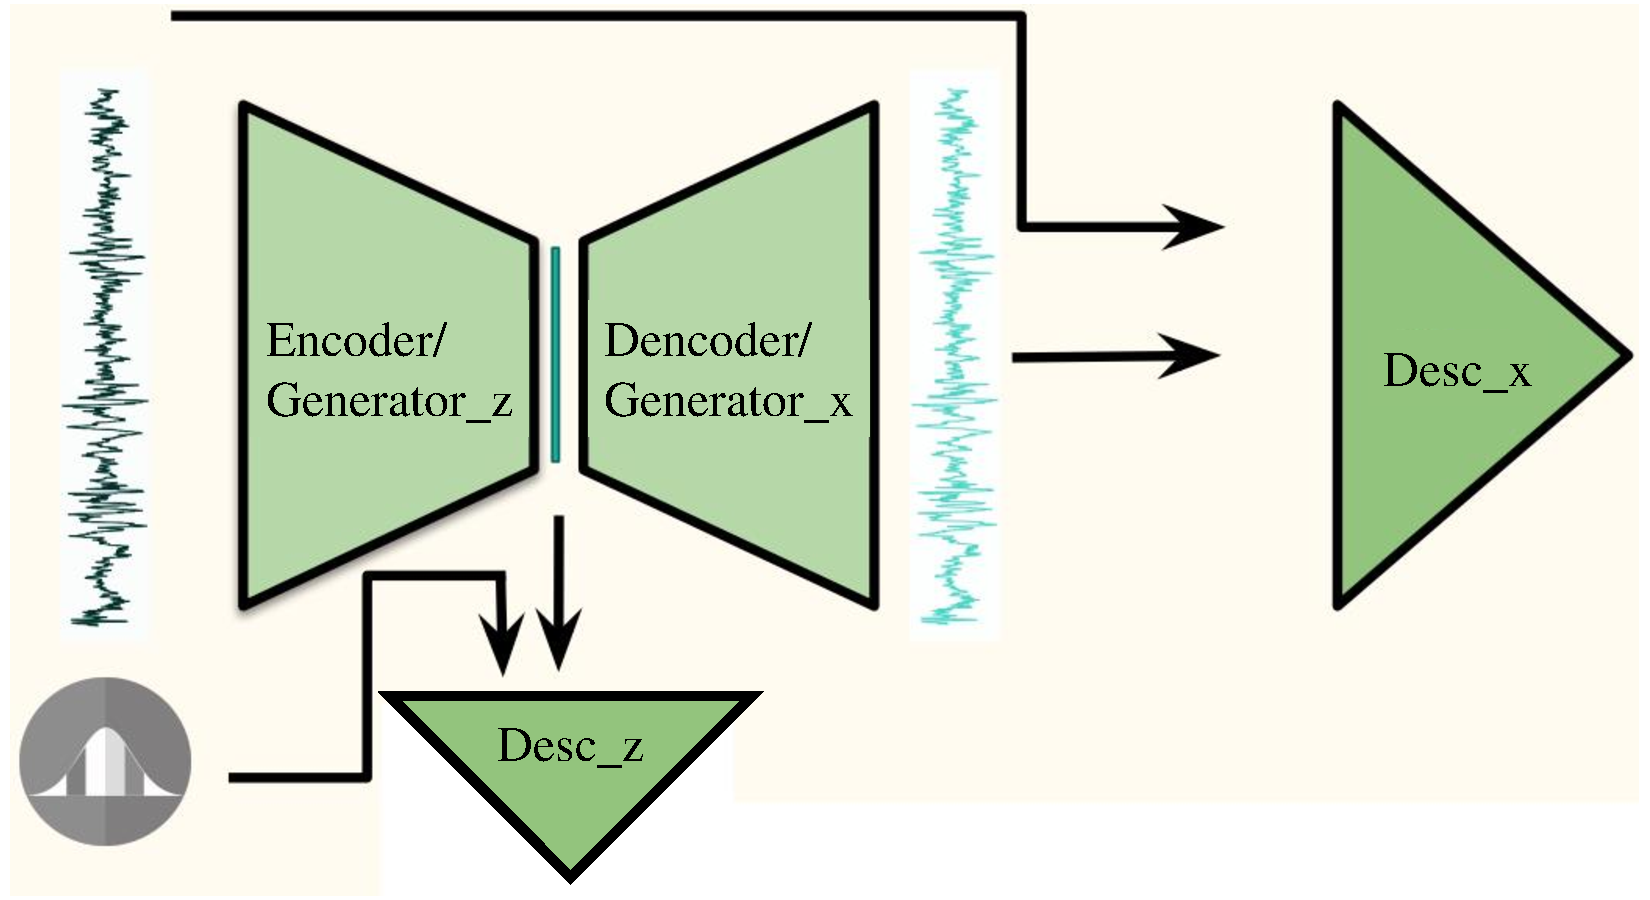
\includegraphics[width=0.9\linewidth]{figures/network_structure.pdf}
	\caption{Proposed network structure.}
	\label{workflow}
\end{figure}
\label{model}


\section{Method}
In this section, we describe the proposed adversarial autoencoder-based anomaly detection method in detail. The main idea is to train the model with only normal data and measure the deviation of test data from the learned distribution with two performance metrics: reconstruction error and distribution distance of latent vectors. Note that here we denote normal data is the data that belong to the period before disease induction procedure, which has nothing to do with mathematical normal distribution.

\subsection{Proposed Model - Amr}
We formulate our task as an unsupervised anomaly detection problem by learning only the distribution of the baseline EEG data through an adverserial autoencoder (AAE). AAE is formed of three sub-networks: encoder, decoder, and discriminator (see Fig. \ref{workflow}). The encoder is trained to map the input data into a lower-dimensional latent space $P(z|X)$, which the decoder uses to reconstruct the input $p(X|z)$. By being trained to discriminate between true samples from the prior distribution and the fake samples generated by the encoder, the discriminator generates a teaching signal to the encoder to generate latent space code that lies within the prior distribution. Specifically the discriminator is trained with the loss function:
\begin{equation}
\mathcal{L}_{D i s}=-\log (\operatorname{Dis}(\mathbf{z}))-\log (1-\operatorname{Dis}(\operatorname{Enc}(\mathbf{X})))
\end{equation}
where $z$ are the true samples from the prior distribution and $X$ are the data samples. On the other hand, the encoder and the decoder are trained with the loss function:
\begin{equation}
\mathcal{L}_{AE}= \left\Vert \mathbf{X} - \operatorname{Dec}(\operatorname{Enc}(\mathbf{X})) \right\Vert^2 -\log (\operatorname{Dis}(\operatorname{Enc}(\mathbf{X})))
\end{equation}

After training, the AAE can be used to scan the query data to look for deviations from the training data distribution. In the data space, anomalous data are expected to have high reconstruction errors and in the latent space, we hypothesize that they will deviate away from the center of the prior distribution used for training.
Input data are 1 second EEG segments collected as described in section \ref{dataset} and sampled at 512 Hz. The encoder model is a simple 5 layer convolutional neural network with kernel size = 5, stride = 2 to consequently downsample the signal, and $2^{(3+k)}$ feature maps per layer $k$. Additionally, we added a final fully connected layer to flexibly map the features of the last convolutional layer to the desired dimension of the latent space, which in our case is 16. The decoder model reconstructs the input from the latent code through a fully connected layer and series of 5 transpose convolutional layers that sequentially upsample the signal and lower the number of feature maps till we reach the 512-dimensional input size.   

\subsection{Cross-validation scheme}
\textbf{I already mentioned it in the data set section.}
yes, i have seen that, but this is confusing for me, because  I think the data set section should only be descriptive of the data, its collection and its preprocessing. I think the model should be described in details before we talk about its training! 
We adopt leave-one-out (LOO) cross validation scheme where we iterate down the list of all rats (seven PPS rats and three control rats) we have and each trial we withhold the data from the rat completely. To be specific, during training, from the PPS group, we only use the data from the BL period, since the model is expected to capture the features in the BL period, such that it could detect signals that do not conform to the learned regularity, which is defined as anomaly. 
To make sure that the model is learning EPG-related features and not the artifacts induced by the long-term recording, we use the data from the control rats, covering weeks of recordings time.   
From the control group, we use the data spanning the whole recording period for training. The discrepancy of time period selections between the PPS group and the control group is due to the fact that it is common in longitudinal recordings, the long-term electrode implantation could cause an increased impedance of the electrode, which causes an increased high frequency component in the EEG signals \cite{straka2018characterizing}. During testing, we take the pre-trained model and scanning over all rat we have from the withheld rat.
% i think the cross validation scheme should be in the experiment part not in the dataset part.

To be specific, 1) we randomly selected 20 hours from each PPS animal from the BL period. 2) We randomly select 100 hours from the whole recording period from control animals. 3) we take non-overlapping one second EEG data as input to the model.



\subsection{The testing process}
After training the full model on the baseline data from 9 out of 10 animals, we tested the ability of the trained model to distinguish between baseline and epileptogenesis periods of the data from the withheld animal using two metrics: reconstruction error ($\mathcal{RE}$) and the distance of the latent code to the origin of the prior distribution ($\mathcal{D}$). 

\begin{equation}
\mathcal{RE(\mathbf{x})}= \left\Vert \mathbf{x} - \operatorname{Dec}(\operatorname{Enc}(\mathbf{x})) \right\Vert^2 
\end{equation}

\begin{equation}
\mathcal{D}(\mathbf{x})= \left\Vert 0 - \operatorname{Enc}(\mathbf{x}) \right\Vert^2
\end{equation}
We set a threshold for these metrics based on the statistics of the training data e.g. $99^{th}$ percentile of the distribution of these metrics computed from the training dataset. In order to aggregate the evidence from longer recording time periods, and in the same time simulate a clinical setting, we compute the average number of surpathreshold segments within a certain time window e.g. 1 hour for both BL and EPG data of the test animal. Consequently, we evaluate the ability of this aggregated metric to distinguish between BL and EPG data by drawing the receiver operating characteristic (ROC) curve, and computing the area under the curve (AUC). We apply this process for the $\mathcal{RE}$ and $\mathcal{D}$ metrics. Moreover, we investigate our hypothesis that a weighted average of both metrics would lead to better classification results. The intuition behind the hypothesis is that anomalous features arising from the epileptogenesis process could be either local (affecting few timepoints), or global (affecting all timepoints of the training segments), and therefore would behave differently in the latent space and in the reconstructed data space.


% \begin{equation}
% \mathcal{D}(\mathbf{p}, \mathbf{z})=\sqrt{\sum_{i=1}^{n}\left(z_{i}-p_{i}\right)^{2}}
% \end{equation}

\subsection{Implementations and training settings}








% 	The model is trained to learn a good compressed representation of the input data $Z$while retaining the 

% 	There three components in our proposed framework: an autoencoder, trained with $\left\Vert x - \hat{x} \right\Vert^2$ that is able to extract the common features of variation from BL recordings and reconstruct them faithfully


% 	There are two sources of anomaly: samples that are poorly reconstructed, i.e., with high reconstruction; the distance between the encoded latent representation distribution to the learned prior.
% 	\subsection{Architecture}
% 	We implemented an adversarial autoencoder for the unsupervised anomaly detection task.
% 	\cite{makhzani2015adversarial}, 
% 	\cite{yer2019detection} - detection of accounting anomalies in the latent space using adversarial autoencoder neural networks: 
% 	\subsection{Naive classifier}
%     \begin{itemize}
%         \item what is the anomaly score for classification
%     \end{itemize}
% 	Put histogram as input to a classifier.

% 	reconstruction error,

% 	distance of current encoded latent vectors to the center of BL distribution
% 	After the network has been trained on only BL data, we scan all the data from the withheld data



\section{Experiment - Amr-Diyuan}

\begin{itemize}
	\item plots: error evolution in one example animal
	\item plot: histogram evolution in one example animal? potentially we could also use the error histogram to so a simple classification.
	\item plot2: error histogram for BL and EPG
	\item table: ROC performance with different metrics
	\item experiment on another data set? We could add the dataset from Massimo, where they also have BL
\end{itemize}

Explanation for sometimes the model have even lower loss in testing data than that in validation data could be linked to the fact that likelihoods from the generative models show a strong bias towards the complexity of the input data \cite{serra2019input, schirrmeister2020understanding, ren2019likelihood}. That is to say the generative model tends to generate lowest likelihoods for qualitatively complex signals, and relatively high likelihoods for simple signals.


\subsection{Ablation Study}
\begin{itemize}
	\item without control rats
	\item change the weights for ae loss weight, reg loss, gen z loss, gen x loss, dc loss? Have enough time? What is the most obvious and promising direction?
	\item visualize the features that have anomalous reconstruction error or latent vector.
\end{itemize}


To further understand different aspects of the proposed method, we perform ablation studies. Specifically, we aim to investigate the effectiveness of different loss components to the final EPG detection task. In this section, we perform ablation studies on components of our proposed network such that we could further understand what exactly are the features that are evolving in EPG that lead the brain to being epileptic.
\begin{itemize}
	\item with only reconstruction error
	\item with only latent z
	\item with supra-threshold events and reconstruction errors
\end{itemize}


\section{Required: Discussion} 

\emph{This is probably the most important section of your paper!  This
	is where you tell us how your work advances our understanding of
	machine learning and healthcare.}  Discuss both technical and
clinical implications, as appropriate.

\paragraph{Limitations}

Explain when your approach may not apply, or things you could not
check.  \emph{Discussing limitations is essential.  Both ACs and
	reviewers have been coached to be skeptical of any work that does
	not consider limitations.}




\bibliography{mlhc2021}



\end{document}
